% This example is from WYATT LLOYD@CACM14 (Don't Settle For Eventual Consistency)
\documentclass{standalone}

\usepackage{tikz}
\usetikzlibrary{positioning, calc}

\begin{document}
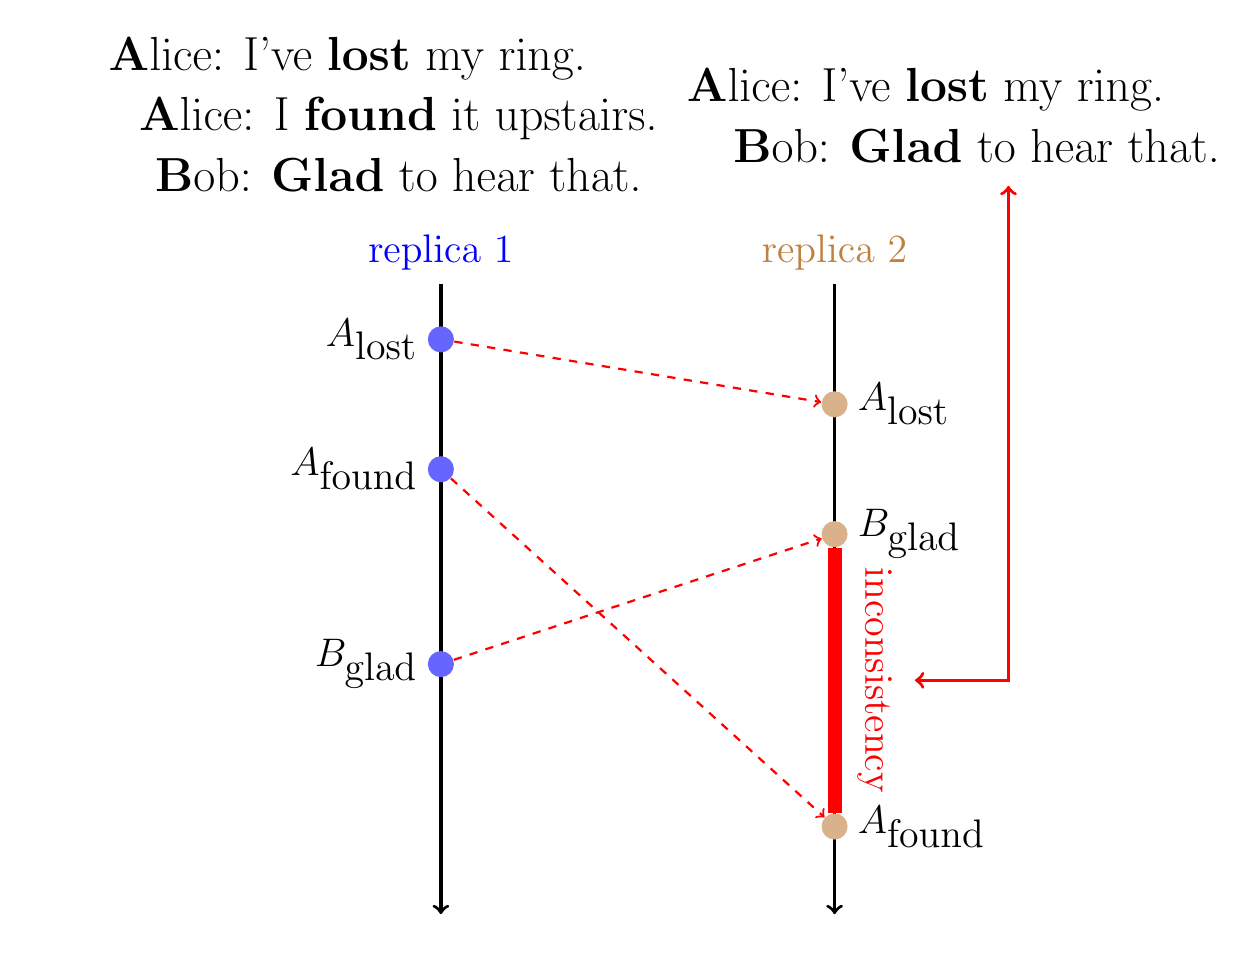
\begin{tikzpicture}
  % replica A at west coast
  \begin{scope}[font = \Large, wnode/.style = {fill = blue!60, circle}]
    \node (west-start) [] at (0,0) {};
    \node (west-end) [below = 8cm of west-start] {};
    \draw [->, very thick] (west-start) to (west-end);

    \node (west-a-lost) [wnode, label = 180: $A_{\textrm{lost}}$] at ($(west-start) !0.10! (west-end)$) {};
    \node (west-a-found) [wnode, label = 180: $A_{\textrm{found}}$] at ($(west-start) !0.30! 
    (west-end)$) {};
    \node (west-b-glad) [wnode, label = 180: $B_{\textrm{glad}}$] at ($(west-start) !0.60! (west-end)$) {};

    % text
    \node (west-text) [above left = 0.8cm and -3.00cm of west-start, align = center, font = \LARGE] {{\bf A}lice: I've {\bf lost} my ring.
    \\ $\qquad$ {\bf A}lice: I {\bf found} it upstairs. 
    \\ $\qquad$ {\bf B}ob: {\bf Glad} to hear that.};

    % replica 1 at west coast
    \node (replica1) [above = -0.20cm of west-start, font = \Large] {\textcolor{blue}{replica 1}};
  \end{scope}

  % replica B at east coast
  \begin{scope}[xshift = 5.0cm, font = \Large, enode/.style = {fill = brown!60, circle}]
    \node (east-start) [] at (0,0) {};
    \node (east-end) [below = 8cm of east-start] {};
    \draw [->, very thick] (east-start) to (east-end);

    \node (east-a-lost) [enode, label = 0: $A_{\textrm{lost}}$] at ($(east-start) !0.20! (east-end)$) {};
    \node (east-b-glad) [enode, label = 0: $B_{\textrm{glad}}$] at ($(east-start) !0.40! 
    (east-end)$) {};
    \node (east-a-found) [enode, label = 0: $A_{\textrm{found}}$] at ($(east-start) !0.85! (east-end)$) {};
    
    % text
    \node (east-text) [above right = 1.0cm and -3.00cm of east-start, align = center, font = \LARGE, outer sep = 5pt] {{\bf A}lice: I've {\bf lost} my ring.  \\ $\qquad$ {\bf B}ob: {\bf Glad} to hear that.};
    
    % replica B at east coast
    \node (replicaB) [above = -0.20cm of east-start, font = \Large] {\textcolor{brown}{replica 2}};
  \end{scope}

  % message-passing and message-reordering
  \begin{scope}[->, thick, dashed, red]
    \draw (west-a-lost) to (east-a-lost);
    \draw (west-a-found) to (east-a-found);
    \draw (west-b-glad) to (east-b-glad);
  \end{scope}

  \begin{scope}[font = \Large]
    % emphasis on data inconsistency
    \draw [line width = 5pt, red] (east-b-glad) -- (east-a-found) node (inconsistency) [above, 
    midway, sloped, outer sep = 5pt] {inconsistency};
    \draw [very thick, red, <->] (inconsistency) -| ($(east-text.south) + (30pt,0)$);
  \end{scope}
\end{tikzpicture}
\end{document}
